\documentclass[conference]{IEEEtran}
\IEEEoverridecommandlockouts
\usepackage{cite}
\usepackage{amsmath,amssymb}
\usepackage{graphicx}
\usepackage{booktabs}
\usepackage{multirow}
\usepackage{xcolor}
\usepackage{tikz}
\usetikzlibrary{arrows.meta,positioning,fit}
\usepackage{url}
\usepackage[hidelinks]{hyperref}

% Figures come from scripts/make_figures.py (Kaggle notebook 06 -> paper_results.zip -> paper/figures/).
% A missing figure renders as a labelled box instead of breaking the build.
\newcommand{\maybefig}[2]{\IfFileExists{figures/#1}{\includegraphics[width=#2]{figures/#1}}%
  {\fbox{\parbox[c][3cm][c]{0.95#2}{\centering\small missing: figures/#1}}}}
\newcommand{\dap}{\Delta\mathrm{AP}}

\begin{document}

\title{Seeing Better Is Not Detecting Better: Benchmarking No-Reference Quality Metrics and Learning Detection-Aware Enhancement Decisions for Underwater Images}

\author{\IEEEauthorblockN{Author Name}
\IEEEauthorblockA{Department of Computer Science and Engineering\\
Manipal Institute of Technology, Manipal, India\\
email@domain}}

\maketitle

\begin{abstract}
Enhanced underwater images are routinely judged by the hand-crafted no-reference (NR) metrics UIQM and UCIQE, and enhancement is routinely applied before object detection. We test both habits on public data under one protocol. First, we benchmark 16 NR image-quality metrics against human opinion scores on UID2021 (960 images, 77 observers) with bootstrap confidence intervals, paired significance tests and intra-scene rank correlation. Only the underwater-trained URanker reaches a Spearman correlation of 0.62. In-air deep metrics fall to near zero when ranking enhancements of the same scene, and UCIQE and URanker are inflated by deliberate over-enhancement. Second, we label every held-out image of a leakage-safe re-split of RUOD, and a duplicate-free subset of DUO, with the change in per-image detection AP caused by five enhancers, measured by a frozen YOLO11 detector and calibrated against a label-noise floor. All five enhancers lower mean AP (by 0.02--0.08 on RUOD and 0.05--0.20 on DUO). A per-image oracle could still gain 0.025 mAP, about ten times what label noise alone produces. A lightweight predictor that sees only the raw image ranks the detection-utility change far better than any NR-IQA metric (Spearman 0.32 vs.\ $\le$0.13). However, selective enhancement driven by it only matches never enhancing, whereas choosing the enhancer with the best NR-IQA gain, as common practice suggests, costs up to 0.17 mAP. We also report that the public re-split of RUOD leaks near-duplicate frames across splits and overlaps heavily with DUO. Code and per-image utility labels are released.
\end{abstract}

\begin{IEEEkeywords}
underwater image enhancement, no-reference image quality assessment, object detection, task-aware quality, benchmark
\end{IEEEkeywords}

% ======================================================================
\section{Introduction}
Light underwater is attenuated in a wavelength-dependent way and scattered by suspended particles. Images therefore show colour casts, low contrast and haze that worsen with depth and turbidity. Hundreds of underwater image enhancement (UIE) methods address this. Because no physically clean reference exists for real underwater scenes, they are usually compared with two hand-crafted NR metrics: UIQM~\cite{panetta2016uiqm} and UCIQE~\cite{yang2015uciqe}. Both combine low-level colourfulness, sharpness, contrast and saturation statistics. Both are known to reward over-processed output~\cite{li2020uieb,li2022limits}.

Two questions follow. \emph{Do these metrics, or the modern deep NR-IQA models that could replace them, agree with human judgement of enhanced underwater images?} Recent evidence is encouraging but thin: Dumic~\textit{et al.}~\cite{dumic2026reliable} report strong correlations for TOPIQ and LIQE on two small datasets enhanced by four methods. \emph{And does enhancement help the downstream task most pipelines care about, object detection?} Wang~\textit{et al.}~\cite{wang2024isuie} and Saleem~\textit{et al.}~\cite{saleem2025influence} find that it generally does not. Awad~\textit{et al.}~\cite{awad2026revisiting} show that an oracle that picks enhanced or raw per image would beat both, and call for metrics that consider quality and detection jointly.

This paper connects the two questions under one reproducible protocol. Our contributions are:
\begin{itemize}
\item A benchmark of 16 NR-IQA metrics (hand-crafted, in-air deep, and underwater-trained) on UID2021~\cite{hou2023uid2021}. It reports correlations with bootstrap CIs, paired significance tests and \emph{intra-scene} rank correlation, plus an over-enhancement stress test that shows which metrics can be gamed.
\item Per-image detection-utility labels for five enhancers on 7{,}000 held-out RUOD images~\cite{fu2023ruod} and 4{,}539 DUO images~\cite{liu2021duo}. The labels come from a frozen detector, are calibrated against a label-noise floor, and use leakage-safe splits built from a near-duplicate analysis that exposes split leakage and RUOD--DUO overlap.
\item A detection-aware predictor that sees only the raw image, compared against NR-IQA metrics as utility predictors, and an evaluation of selective-enhancement policies at dataset level. It includes an oracle upper bound and a noise-only control that separates real headroom from label noise.
\end{itemize}
Task-aware quality assessment itself is not new~\cite{awad2026revisiting}. Our delta is a \emph{learned, deployable, raw-image-only} predictor of per-image detection utility, evaluated jointly with a human-opinion benchmark and across datasets.

% ======================================================================
\section{Related Work}
\textbf{Evaluating enhanced underwater images.} UIQM~\cite{panetta2016uiqm} and UCIQE~\cite{yang2015uciqe} remain the default NR metrics. UIEB~\cite{li2020uieb} provides quasi-references chosen by human voting rather than true clean images. Li and Cavallaro~\cite{li2022limits} concluded that none of the NR measures they evaluated satisfactorily rates enhanced underwater images. Subjective datasets such as UID2021~\cite{hou2023uid2021} and SAUD~\cite{jiang2022saud} provide mean opinion scores (MOS) for many enhancers per scene. URanker~\cite{guo2023uranker} learns to rank enhanced underwater images.

\textbf{Deep NR-IQA.} General-purpose models such as MUSIQ~\cite{ke2021musiq}, CLIP-IQA~\cite{wang2023clipiqa}, TOPIQ~\cite{chen2024topiq}, LIQE~\cite{zhang2023liqe}, MANIQA~\cite{yang2022maniqa}, TReS~\cite{golestaneh2022tres}, ARNIQA~\cite{agnolucci2024arniqa} and QualiCLIP~\cite{agnolucci2024qualiclip} are trained on in-air distortions (compression, blur, noise, authentic camera artefacts). These differ physically from underwater degradation.

\textbf{Enhancement for detection.} Wang~\textit{et al.}~\cite{wang2024isuie} trained 133 detectors on raw and enhanced data and found that enhancement does not reliably help. Saleem~\textit{et al.}~\cite{saleem2025influence} analysed effects per image and found that over-enhancement in particular degrades detection. Awad~\textit{et al.}~\cite{awad2026revisiting} proposed a per-image evaluation protocol and an oracle mixed-set upper bound. We follow their per-image view, but learn a predictor instead of using an oracle, and report the gap between the two.

% ======================================================================
\section{Method}
\begin{figure}[t]
\centering
\resizebox{\columnwidth}{!}{%
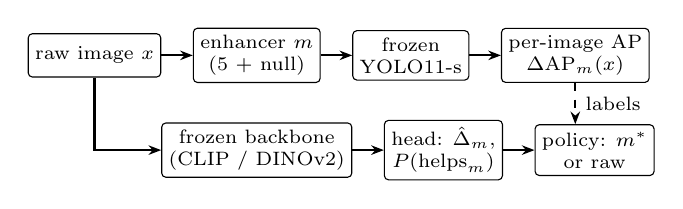
\begin{tikzpicture}[node distance=3mm and 4mm, every node/.style={font=\scriptsize},
  box/.style={draw, rounded corners=1.5pt, align=center, inner sep=2.5pt, minimum height=5.5mm},
  arr/.style={-{Stealth[length=1.6mm]}, thick}]
\node[box] (raw) {raw image $x$};
\node[box, right=of raw] (enh) {enhancer $m$\\(5 + null)};
\node[box, right=of enh] (det) {frozen\\YOLO11-s};
\node[box, right=of det] (ap) {per-image AP\\$\dap_m(x)$};
\node[box, below=5mm of enh] (bb) {frozen backbone\\(CLIP / DINOv2)};
\node[box, right=of bb] (head) {head: $\hat{\Delta}_m$,\\$P(\text{helps}_m)$};
\node[box, right=of head] (pol) {policy: $m^*$\\or raw};
\draw[arr] (raw) -- (enh); \draw[arr] (enh) -- (det); \draw[arr] (det) -- (ap);
\draw[arr] (raw.south) |- (bb.west); \draw[arr] (bb) -- (head); \draw[arr] (head) -- (pol);
\draw[arr, dashed] (ap.south) -- node[right, align=left] {labels} (pol.north -| ap.south);
\end{tikzpicture}}
\caption{Pipeline. Top: detection-utility labels. Each raw image is enhanced in memory, detected by a detector trained on raw images only, and scored against ground truth. Bottom: a deployable predictor sees only the raw image and decides whether, and how, to enhance.}
\label{fig:pipeline}
\end{figure}

\subsection{Data and leakage-safe splits}
\textbf{UID2021}~\cite{hou2023uid2021} contains 60 raw images from six degradation types (bluish, blue-green, greenish, hazy, low-light, turbid), each enhanced by 15 methods: 960 images at $512\times384$, with MOS from 77 observers in the current public release.

\textbf{RUOD}~\cite{fu2023ruod} (14{,}000 images, 74{,}904 boxes, 10 classes) and \textbf{DUO}~\cite{liu2021duo} (7{,}782 images, 74{,}515 boxes, 4 classes) were taken from the YOLO-format ODverse33 copy~\cite{odverse33}. DUO's classes (holothurian, echinus, scallop, starfish) share their ids with RUOD's first four classes, so a RUOD detector can be tested on DUO directly.

We hashed every image with a 256-bit difference hash and linked pairs within Hamming distance 32. Visual inspection showed that pairs up to distance 26 are frames of the same video. Between 27 and 32 a few low-texture false matches appear; these only make groups conservatively large. We found 7{,}979 near-duplicate pairs: \textbf{3{,}252 link RUOD to DUO}, and \textbf{1{,}609 cross the official RUOD splits}. We therefore re-split RUOD by connected duplicate group into det-train/det-val (45\%/5\%) for the detector and pred-train/pred-val/pred-test (30\%/10\%/10\%) for the predictor. The detector never sees the pred-* images. For cross-dataset testing we keep only the 4{,}539 labelled DUO images that share no group with RUOD (\emph{DUO-clean}).

\subsection{NR-IQA benchmark and stress test}
We evaluate 16 metrics through IQA-PyTorch~\cite{chen2022iqapytorch}, using their released weights and no fine-tuning:
\begin{itemize}
\item hand-crafted: UIQM, UCIQE (two implementations), NIQE~\cite{mittal2013niqe}, BRISQUE~\cite{mittal2012brisque};
\item in-air deep: MUSIQ, CLIP-IQA, CLIP-IQA+, TOPIQ-NR, LIQE, LIQE-mix, MANIQA, TReS, ARNIQA, QualiCLIP;
\item underwater-trained: URanker.
\end{itemize}
UIQM and UCIQE were re-implemented from the original formulas. Our UIQM block computation matches a widely used reference port exactly.

We report SRCC, KRCC and PLCC (after the VQEG four-parameter logistic mapping~\cite{vqeg2000}), each with a 95\% percentile-bootstrap CI~\cite{efron1994bootstrap}, and a paired bootstrap test against the best metric. Because UID2021 contains 16 versions of every scene, we also report the mean \emph{intra-scene} SRCC: the correlation within each scene's 16 images. This measures what a metric is actually used for, ranking enhancements of the same image.

The stress test applies four controlled distortions (contrast stretch, saturation boost, unsharp masking, red over-compensation) at strengths $s\in\{0,0.25,\dots,3\}$ to the 60 raw images. For each metric it reports the Spearman correlation between score and $s$; a metric that rises monotonically with heavy processing is gameable.

\subsection{Detection-utility labels}
A YOLO11-s detector~\cite{jocher2023ultralytics} is trained on det-train only (640\,px, 100 epochs) and then frozen; this is protocol (a), which isolates the effect of preprocessing. For each held-out image, the raw image is resized to a long side of 1280\,px and enhanced in memory by CLAHE~\cite{zuiderveld1994clahe}, gray-world~\cite{buchsbaum1980grayworld}, UDCP~\cite{drews2013udcp}, fusion~\cite{ancuti2018fusion} and FUnIE-GAN~\cite{islam2020funie}. The first four are our compact re-implementations; FUnIE-GAN uses the official code and weights. All variants are detected, and each is scored with COCO-style per-image AP$_{50:95}$~\cite{lin2014coco}. This gives $\dap_m(x)=\mathrm{AP}(m(x))-\mathrm{AP}(x)$.

To calibrate label noise we add a \emph{null} enhancer: a visually invisible JPEG $q{=}95$ re-encode. We set $\tau$ to the 95th percentile of $|\dap_{\text{null}}|$ on pred-train ($\tau=0.050$) and define $\text{helps}_m(x)=[\dap_m(x)>\tau]$. All detections are stored, so the dataset-level mAP of any per-image policy can be computed without re-running the detector. Our AP implementation matches Ultralytics' mAP to within 0.005 on identical predictions.

\subsection{Detection-aware predictor and policies}
The predictor sees only the raw image, squashed to $224\times224$ and passed through a frozen backbone: CLIP ViT-B/32~\cite{radford2021clip}, DINOv2 ViT-S/14~\cite{oquab2024dinov2}, ResNet-18~\cite{he2016resnet}, or CLIP+DINOv2. Three heads predict the per-method $\hat{\Delta}_m$ and $P(\text{helps}_m)$:
\begin{itemize}
\item ridge regression;
\item per-method logistic regression;
\item a multi-task MLP (one 256-unit hidden layer) trained with Smooth-L1 on $\dap$, class-balanced BCE on $\text{helps}$, and a pairwise logistic ranking loss, as a 3-seed ensemble with early stopping on pred-val SRCC.
\end{itemize}
NR-IQA baselines use either raw-image quality, $-Q(x)$ (``enhance images that look bad''), or the quality gain $Q(m(x))-Q(x)$, for UIQM, UCIQE, TOPIQ, LIQE and URanker.

A policy picks $m^*(x)=\arg\max_m \hat{s}_m(x)$ and enhances with $m^*$ only if $\hat{s}_{m^*}(x)>\delta$; otherwise it keeps the raw image. The margin $\delta$ is tuned on pred-val only. We compare against:
\begin{itemize}
\item always-raw and always-$m$;
\item the per-image \emph{oracle} (best true AP);
\item a \emph{noise oracle} that chooses per image between raw and the null re-encode, which shows how much gain pure label noise produces;
\item the ``naive'' NR-IQA practice of always applying the enhancer with the largest quality gain.
\end{itemize}

% ======================================================================
\section{Results}
\subsection{Reference detector}
The frozen detector reaches mAP$_{50}$/mAP$_{50:95}$ of 0.811/0.569 on det-val, 0.798/0.556 on the held-out pred-test, and 0.639/0.387 on DUO-clean. The DUO drop comes mainly from echinus recall (0.54 at 0.96 precision; about 9 small urchins per image). Recomputed from our stored detections at the 1280\,px working resolution, the scores are 0.799/0.561 (RUOD pred-*) and 0.644/0.402 (DUO-clean), so the labelling protocol does not alter the detector's behaviour.

\subsection{NR-IQA vs.\ human opinion (UID2021)}
\begin{table}[t]
\centering
\caption{NR-IQA metrics vs.\ MOS on UID2021 (960 images). 95\% bootstrap CI on SRCC; ``intra'' is the mean SRCC within each of the 60 scenes. Every metric is significantly below URanker (paired bootstrap, $p<0.005$).}
\label{tab:o1}
\setlength{\tabcolsep}{3.2pt}
\footnotesize
\begin{tabular}{@{}lccccc@{}}
\toprule
Metric & SRCC & 95\% CI & PLCC & KRCC & Intra \\
\midrule
URanker~\cite{guo2023uranker} & \textbf{0.623} & [0.581, 0.665] & \textbf{0.640} & \textbf{0.445} & \textbf{0.578} \\
LIQE-mix & 0.484 & [0.434, 0.529] & 0.480 & 0.334 & 0.381 \\
LIQE~\cite{zhang2023liqe} & 0.482 & [0.431, 0.528] & 0.499 & 0.330 & 0.401 \\
MUSIQ~\cite{ke2021musiq} & 0.403 & [0.349, 0.458] & 0.422 & 0.276 & 0.303 \\
ARNIQA~\cite{agnolucci2024arniqa} & 0.388 & [0.332, 0.443] & 0.408 & 0.268 & 0.289 \\
UCIQE~\cite{yang2015uciqe} & 0.334 & [0.275, 0.388] & 0.369 & 0.227 & 0.351 \\
UIQM~\cite{panetta2016uiqm} & 0.325 & [0.272, 0.379] & 0.323 & 0.218 & 0.293 \\
TOPIQ-NR~\cite{chen2024topiq} & 0.316 & [0.257, 0.373] & 0.330 & 0.212 & 0.167 \\
UCIQE (legacy port) & 0.312 & [0.251, 0.367] & 0.366 & 0.213 & 0.386 \\
CLIP-IQA+ & 0.298 & [0.238, 0.358] & 0.347 & 0.201 & 0.068 \\
TReS~\cite{golestaneh2022tres} & 0.290 & [0.230, 0.344] & 0.306 & 0.194 & 0.070 \\
QualiCLIP~\cite{agnolucci2024qualiclip} & 0.249 & [0.187, 0.313] & 0.276 & 0.169 & 0.022 \\
MANIQA~\cite{yang2022maniqa} & 0.214 & [0.152, 0.273] & 0.241 & 0.142 & $-$0.090 \\
CLIP-IQA~\cite{wang2023clipiqa} & 0.190 & [0.129, 0.254] & 0.204 & 0.129 & 0.021 \\
NIQE~\cite{mittal2013niqe} & 0.158 & [0.095, 0.215] & 0.177 & 0.106 & 0.074 \\
BRISQUE~\cite{mittal2012brisque} & 0.034 & [$-$0.023, 0.095] & 0.072 & 0.022 & $-$0.056 \\
\bottomrule
\end{tabular}
\end{table}

\begin{figure}[t]
\centering
\maybefig{fig_o1_srcc.pdf}{\columnwidth}
\caption{SRCC with MOS (bars, 95\% CI) and mean intra-scene SRCC (diamonds) on UID2021. In-air deep metrics keep a moderate global correlation but cannot rank the 16 versions of one scene.}
\label{fig:o1}
\end{figure}

Table~\ref{tab:o1} and Fig.~\ref{fig:o1} show three findings.

\emph{First}, the only metric trained on underwater enhancement, URanker, is clearly best (SRCC 0.62, intra-scene 0.58). The best in-air models (LIQE, MUSIQ, ARNIQA) reach 0.39--0.48.

\emph{Second}, intra-scene SRCC separates the metrics far more sharply than global SRCC. CLIP-IQA(+), TReS, QualiCLIP and MANIQA fall to between $-0.09$ and $0.07$ when asked to rank enhancements of the \emph{same} image: their global correlation comes mostly from differences between scenes. TOPIQ-NR reaches only 0.32 globally and 0.17 within scenes. That is far below the $\approx$0.8 reported on a four-method study~\cite{dumic2026reliable}, so conclusions drawn from few enhancers do not transfer to UID2021's 15.

\emph{Third}, UIQM and UCIQE reach only 0.33 here, below the 0.54/0.60 that the UID2021 authors report~\cite{hou2023uid2021}. We verified that all 960 image--MOS pairs align (matching the table's own scene labels) and that per-method mean MOS is sensible (UWCNN 1.56 $<$ raw 1.88 $<\dots<$ UWB-VCSE 6.78). The shortfall is uniform across the six degradation types. Two explanations remain: the public MOS was revised from 52 to 77 observers, and the original release is no longer accessible; or the original MATLAB implementations differ from ours.

\subsection{Over-enhancement stress test}
\begin{table}[t]
\centering
\caption{Spearman correlation between metric score and distortion strength ($s=0\to3$), mean over the 60 UID2021 raw images. Large positive values indicate a gameable metric.}
\label{tab:o2}
\footnotesize
\begin{tabular}{@{}lcccc@{}}
\toprule
Metric & Contrast & Red shift & Saturation & Unsharp \\
\midrule
UCIQE & \textbf{0.91} & $-$0.01 & \textbf{0.76} & \textbf{1.00} \\
URanker & \textbf{0.89} & $-$0.51 & $-$0.86 & \textbf{1.00} \\
MUSIQ & 0.08 & $-$0.10 & $-$0.63 & \textbf{0.68} \\
TOPIQ-NR & $-$0.34 & $-$0.01 & $-$0.52 & \textbf{0.60} \\
LIQE & 0.28 & $-$0.18 & $-$0.47 & $-$0.10 \\
UIQM & $-$0.77 & $-$0.30 & $-$0.73 & $-$0.09 \\
\bottomrule
\end{tabular}
\end{table}

\begin{figure*}[t]
\centering
\maybefig{fig_o2_sweeps.pdf}{\textwidth}
\caption{Mean change of each metric relative to the unprocessed image, in units of the metric's standard deviation, as distortion strength grows.}
\label{fig:o2}
\end{figure*}

UCIQE rises almost monotonically with contrast, saturation and sharpening (Table~\ref{tab:o2}, Fig.~\ref{fig:o2}). It can be gamed by exactly the over-processing it is used to judge. URanker, the best metric against MOS, is also inflated by contrast stretching and unsharp masking, though not by colour distortion. MUSIQ and TOPIQ reward over-sharpening. Over this heavy range, UIQM and LIQE do not inflate monotonically. Small-strength inflation, such as UIQM under mild red over-compensation, can hide inside a negative overall correlation.

\subsection{Does enhancement help detection?}
\begin{table}[t]
\centering
\caption{Mean per-image AP$_{50:95}$ and change vs.\ raw. ``helps''/``hurts'' count $\dap>0$ / $<0$ \emph{before} noise calibration.}
\label{tab:o3}
\setlength{\tabcolsep}{2.6pt}
\footnotesize
\begin{tabular}{@{}lcccccc@{}}
\toprule
 & \multicolumn{3}{c}{RUOD pred-* (7{,}000)} & \multicolumn{3}{c}{DUO-clean (4{,}539)} \\
\cmidrule(lr){2-4}\cmidrule(lr){5-7}
Method & $\dap$ & helps & hurts & $\dap$ & helps & hurts \\
\midrule
raw (AP) & \multicolumn{3}{c}{0.673} & \multicolumn{3}{c}{0.531} \\
Null (JPEG $q$95) & $-$0.001 & 21\% & 22\% & $-$0.001 & 24\% & 29\% \\
CLAHE & $-$0.022 & 27\% & 50\% & $-$0.046 & 33\% & 64\% \\
UDCP & $-$0.041 & 24\% & 54\% & $-$0.078 & 26\% & 71\% \\
FUnIE-GAN & $-$0.066 & 21\% & 61\% & $-$0.107 & 23\% & 75\% \\
Gray-world & $-$0.075 & 20\% & 60\% & $-$0.094 & 26\% & 72\% \\
Fusion & $-$0.083 & 20\% & 62\% & $-$0.199 & 14\% & 84\% \\
\bottomrule
\end{tabular}
\end{table}

\begin{figure}[t]
\centering
\maybefig{fig_o3_delta.pdf}{\columnwidth}
\caption{Distribution of per-image $\dap$ on RUOD pred-*. The grey band is the label-noise floor ($\pm\tau$) estimated from the null re-encode.}
\label{fig:o3}
\end{figure}

Every enhancer lowers mean detection AP (Table~\ref{tab:o3}, Fig.~\ref{fig:o3}), and more so on DUO, which is out of distribution for the detector. This agrees with~\cite{wang2024isuie,saleem2025influence}. The null re-encode is the crucial control. It ``helps'' 21--24\% of images, about as often as the enhancers do, so the sign of $\dap$ alone is mostly noise. After calibration ($\dap>\tau=0.05$), each enhancer helps about 11\% of RUOD images (9--19\% on DUO). That is a non-degenerate but minority signal.

\subsection{Predicting detection utility from the raw image}
\begin{table}[t]
\centering
\caption{Predicting the per-image utility change (mean over five enhancers). SRCC: predicted vs.\ true $\dap$; AUROC/BA: $\text{helps}_m$ classification (BA threshold tuned on pred-val). Nothing is tuned on DUO.}
\label{tab:o4}
\setlength{\tabcolsep}{2.4pt}
\footnotesize
\begin{tabular}{@{}lccccc@{}}
\toprule
 & \multicolumn{3}{c}{RUOD pred-test} & \multicolumn{2}{c}{DUO-clean} \\
\cmidrule(lr){2-4}\cmidrule(lr){5-6}
Predictor & SRCC & AUROC & BA & SRCC & AUROC \\
\midrule
MLP, CLIP & \textbf{0.319} & 0.597 & 0.562 & \textbf{0.174} & 0.597 \\
MLP, CLIP+DINOv2 & 0.314 & 0.598 & \textbf{0.576} & 0.172 & \textbf{0.602} \\
MLP, ResNet-18 & 0.311 & 0.597 & 0.550 & 0.158 & 0.597 \\
MLP, DINOv2 & 0.308 & 0.578 & 0.545 & 0.156 & 0.587 \\
MLP, CLIP, no rank loss & 0.319 & 0.595 & 0.563 & 0.168 & 0.596 \\
Logistic, CLIP & -- & 0.596 & 0.567 & -- & 0.593 \\
Ridge, CLIP & 0.315 & 0.519 & 0.506 & 0.154 & 0.483 \\
\midrule
$Q(m(x))-Q(x)$, UCIQE & 0.133 & 0.532 & 0.532 & $-$0.015 & 0.442 \\
$Q(m(x))-Q(x)$, UIQM & 0.026 & 0.515 & 0.518 & $-$0.139 & 0.466 \\
$Q(m(x))-Q(x)$, TOPIQ & $-$0.029 & 0.491 & 0.507 & 0.003 & 0.469 \\
$Q(m(x))-Q(x)$, LIQE & $-$0.130 & 0.486 & 0.502 & $-$0.003 & 0.446 \\
$Q(m(x))-Q(x)$, URanker & $-$0.182 & 0.494 & 0.509 & $-$0.025 & 0.484 \\
$-Q(x)$, LIQE & $-$0.235 & 0.513 & 0.518 & $-$0.026 & 0.598 \\
$-Q(x)$, TOPIQ & $-$0.212 & 0.528 & 0.513 & $-$0.020 & 0.593 \\
$-Q(x)$, URanker & $-$0.223 & 0.499 & 0.508 & $-$0.118 & 0.503 \\
\bottomrule
\end{tabular}
\end{table}

Learned raw-only predictors rank the utility change far better than any NR-IQA signal (Table~\ref{tab:o4}): SRCC 0.31--0.32 on RUOD and 0.16--0.17 on DUO, against at most 0.13. The quality \emph{gain} of an enhancement, the quantity practitioners optimise, is uncorrelated or negatively correlated with its detection gain for every metric, including URanker. Raw-image quality correlates in the \emph{opposite} direction to the usual intuition. For TOPIQ, LIQE and URanker, $-Q(x)$ has SRCC $\approx-0.22$: enhancement hurts detection \emph{more} on images that look worse.

The backbone and the ranking loss barely matter (SRCC 0.31--0.32), which suggests the limit is the signal, not model capacity. On DUO, raw LIQE/TOPIQ scores match the learned classifiers' AUROC ($\approx$0.60) but carry no ranking information.

\subsection{Selective enhancement}
% UPDATE after notebook 06: switch to the dataset-mAP-tuned policies (policies_*_map.csv, fig_o5_policies_map.pdf)
\begin{table}[t]
\centering
\caption{Dataset mAP$_{50:95}$ of enhancement policies. Margins tuned on RUOD pred-val. Bracketed: 95\% paired-bootstrap CI of the change vs.\ always-raw.}
\label{tab:o5}
\setlength{\tabcolsep}{2.6pt}
\footnotesize
\begin{tabular}{@{}lcccc@{}}
\toprule
 & \multicolumn{2}{c}{RUOD pred-test} & \multicolumn{2}{c}{DUO-clean} \\
\cmidrule(lr){2-3}\cmidrule(lr){4-5}
Policy & mAP & $\Delta$ & mAP & $\Delta$ \\
\midrule
Always raw & 0.5548 & -- & 0.4020 & -- \\
Always best enhancer & 0.5299 & $-$0.025 & 0.3420 & $-$0.060 \\
Always worst enhancer & 0.4550 & $-$0.100 & 0.1946 & $-$0.207 \\
NR-IQA choice, UCIQE & 0.5087 & $-$0.046 & 0.3363 & $-$0.066 \\
NR-IQA choice, TOPIQ & 0.4655 & $-$0.089 & 0.2279 & $-$0.174 \\
NR-IQA, tuned margin & 0.5541 & $-$0.001 & 0.3904 & $-$0.012 \\
Learned (ours) & 0.5551 & +0.000 & 0.4020 & 0.000 \\
 & \multicolumn{2}{r}{\scriptsize{}[$-$0.0002, 0.0007]} & & \\
Noise oracle (control) & 0.5572 & +0.002 & 0.4036 & +0.002 \\
Oracle (upper bound) & 0.5801 & +0.025 & 0.4233 & +0.021 \\
\bottomrule
\end{tabular}
\end{table}

\begin{figure*}[t]
\centering
\IfFileExists{figures/fig_o5_policies_map.pdf}{\maybefig{fig_o5_policies_map.pdf}{\textwidth}}{\maybefig{fig_o5_policies.pdf}{\textwidth}}
\caption{Change in dataset mAP$_{50:95}$ relative to always using the raw image, for fixed, NR-IQA-driven, learned and oracle policies.}
\label{fig:o5}
\end{figure*}

The per-image oracle gains 0.025 (RUOD) and 0.021 (DUO) mAP over always-raw, about ten times the noise oracle (0.002). There is real headroom. The learned policy, with its margin chosen on validation, enhances only 0--3\% of images. It therefore matches always-raw (+0.0003, CI includes zero) and beats every always-enhance policy by 0.025--0.06 mAP (Table~\ref{tab:o5}, Fig.~\ref{fig:o5}). The common practice of applying the enhancer with the best NR-IQA gain is harmful: it costs 0.046--0.089 mAP on RUOD and 0.066--0.174 on DUO.

The learned predictor's ranking signal (SRCC 0.32, AUROC 0.60) is thus too weak to pick out the $\approx$11\% of images that benefit, with enough precision to outweigh the losses on the rest.

% ======================================================================
\section{Discussion and Limitations}
\textbf{Detector dependence.} Utility labels come from a detector trained on raw images (protocol (a)), for which enhanced inputs are slightly out of distribution. This isolates the preprocessing effect but may overstate harm. Retraining with enhancement augmentation (protocol (b)) is the natural sensitivity check and is left for future work.

\textbf{Enhancers.} Four of the five enhancers are our compact re-implementations, and our fusion port is untuned. TensorFlow-1 methods such as Water-Net and Ucolor were excluded for reproducibility.

\textbf{Human data.} The benchmark uses one MOS dataset, whose released scores differ from those in its paper. The stress test establishes score inflation, but not human preference at each strength; a small paired-comparison study would close that gap.

\textbf{Per-image AP} is noisy for images with few objects. We control for this with the null enhancer and $\tau$ rather than removing it.

% ======================================================================
\section{Conclusion}
Whether an enhanced underwater image looks better, by human or by metric, says little about whether a detector sees it better. On UID2021, only an underwater-trained ranker tracks human opinion reasonably well. In-air deep metrics cannot rank enhancements of one scene, and the de facto metric UCIQE is gameable. For detection, every enhancer we tested hurts on average. Selecting enhancement by NR-IQA gain hurts more, while a learned raw-image predictor at least avoids the harm. Per-image headroom exists, about ten times the noise level, but neither NR-IQA nor frozen-feature predictors capture it yet. We release the leakage-safe splits, the noise-calibrated per-image utility labels and all code, so that detection-aware enhancement can be measured rather than assumed.

\bibliographystyle{IEEEtran}
\bibliography{refs}

\end{document}
